\subsection{POC 2: Auto-Complete for Conference Registration in Indico}

The second prototype aims at connecting Solid with the conference registration module in Indico. When registering for a conference an \gls{html} form is presented with fields previously defined by the conference manager, who deemed those fields necessary. A form always contains personal information of name and email address, but is not limited to it and can even range to more sensible information such as copies of personal identification documents. Information of this type has perfect motivation to remain in the hand of the owner and not be stored in a remote data store, uncontrollable and unknown to the registrants.

Therefore, the aim is to extend the registration module to allow storage in a data pod, where the user has full control and can handle the data to their own liking.

\subsubsection{Architectural Analysis and Synthesis}\mbox{}\\

\paragraph{System Description}\mbox{}\\
\paragraph{Features}\mbox{}\\
\paragraph{Context Diagram}\mbox{}\\
\paragraph{Sequence Diagram}\mbox{}\\

\begin{figure}[H]
    \centering
    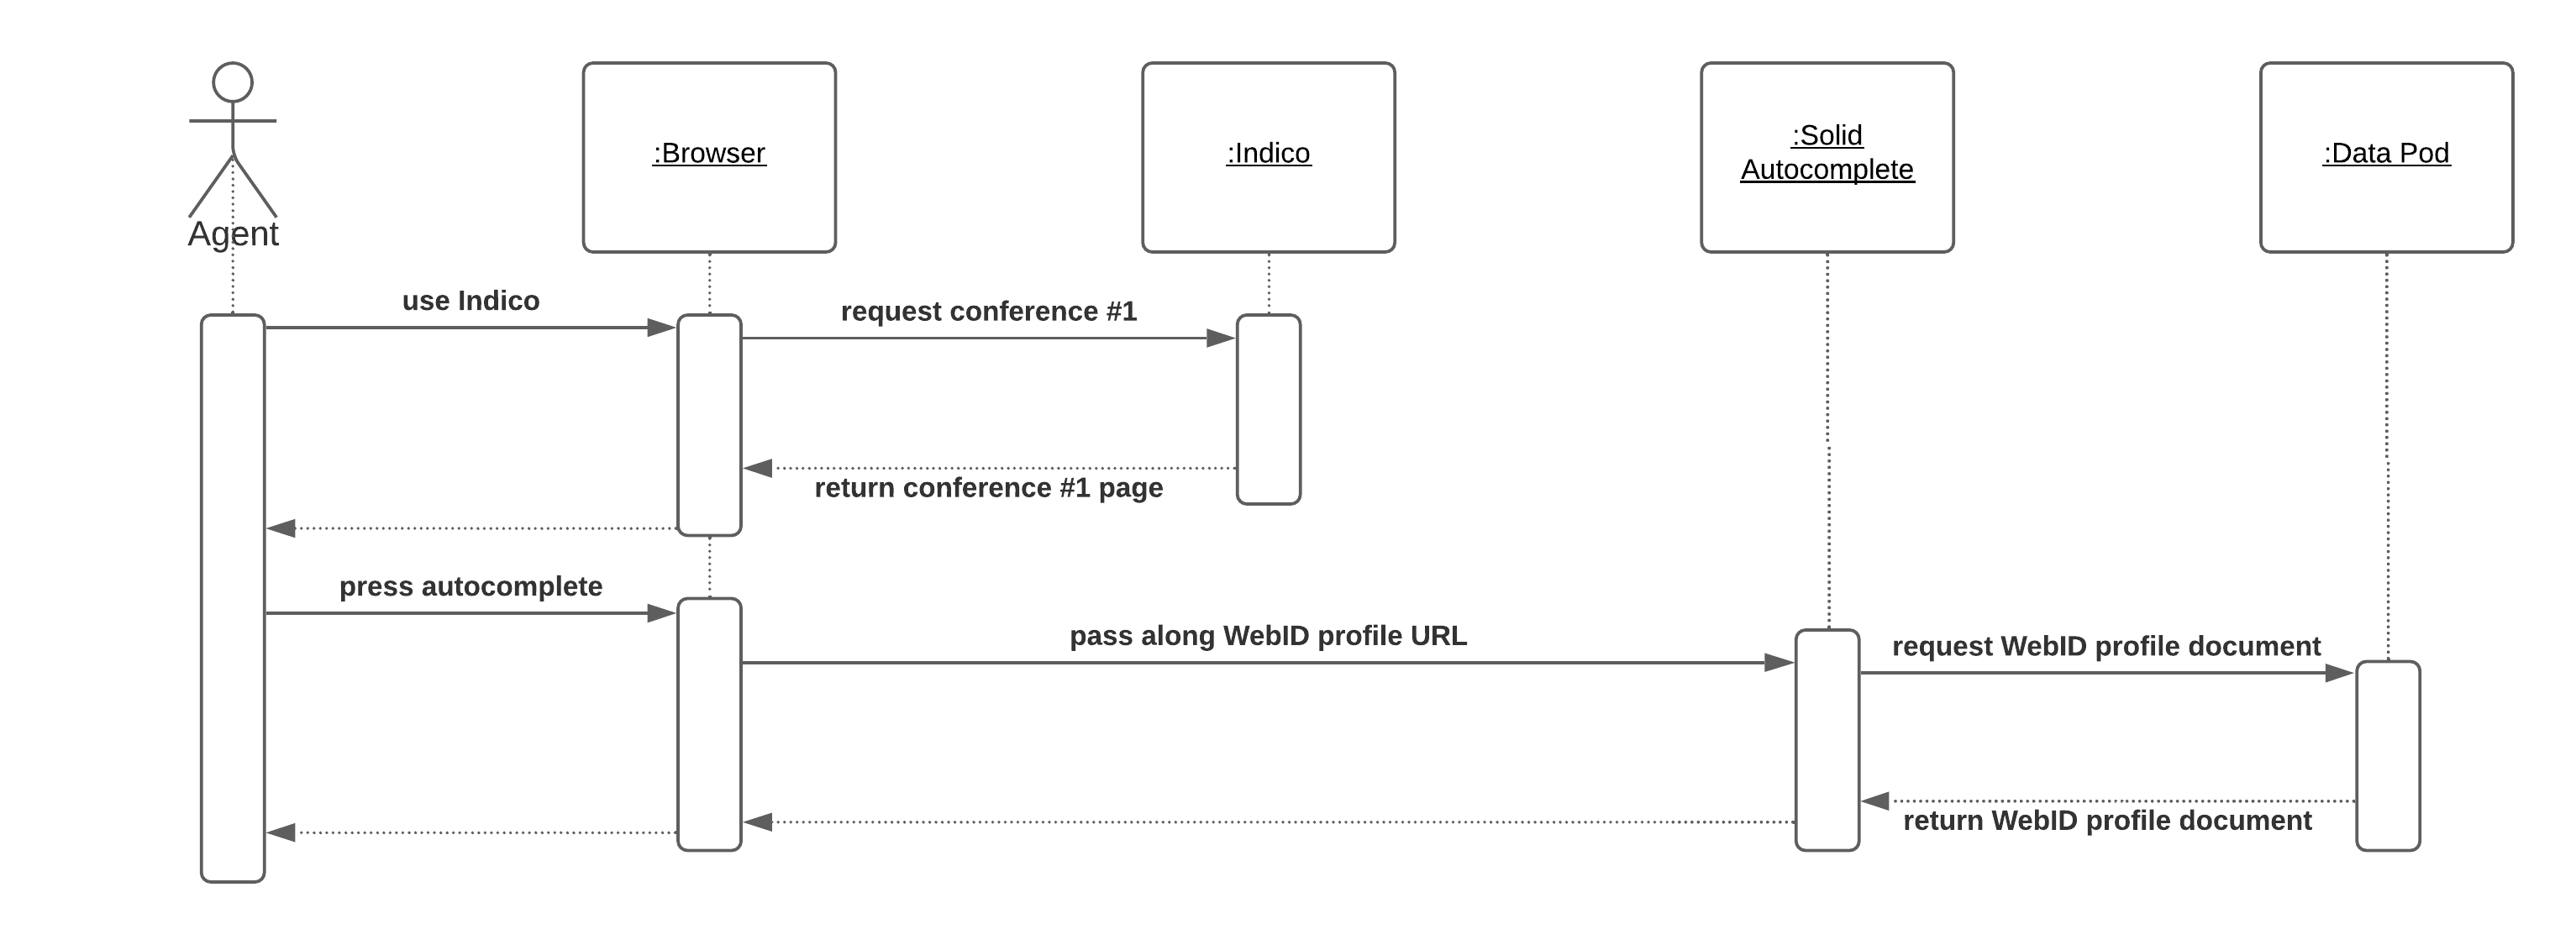
\includegraphics[width=\textwidth]{prototype/graphs/poc-conference_registration-autocomplete-sequence_diagram.png}
    \caption{Sequence diagram showing the sequential process through posting a comment.}
    \label{fig:poc-conference_registration-autocomplete-sequence_diagram}
\end{figure}

\paragraph{Stakeholders}\mbox{}\\
\paragraph{Drivers}\mbox{}\\

\subsubsection{Design}\mbox{}\\

TODO:
1st iteration, save data in pod
2nd iteration, only pull data from pod

TODO: Include these somehow:

\begin{figure}
    \centering
    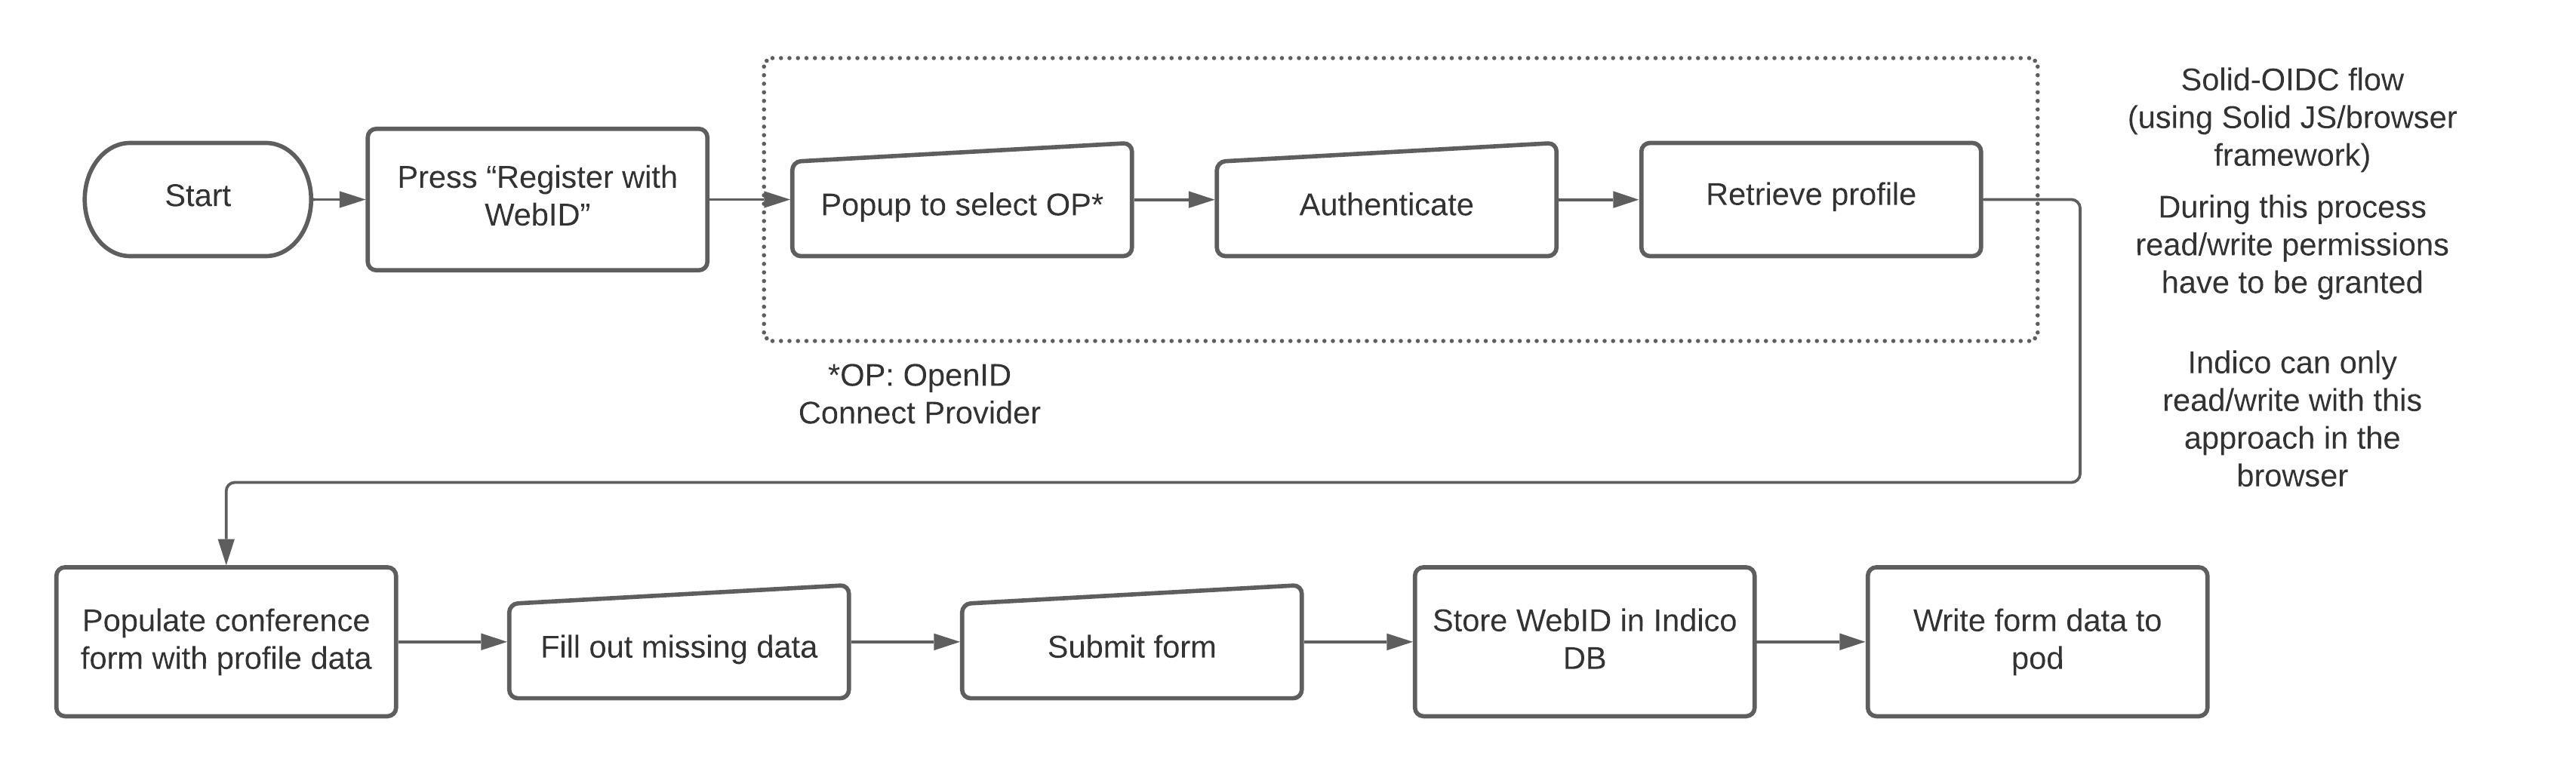
\includegraphics[width=0.6\textwidth]{prototype/graphs/poc-conference_registration_flow-client_side-sideways.jpeg}
    \caption{TODO:}
    \label{fig:poc-conference_registration_flow-client_side-sideways}
\end{figure}

\begin{figure}
    \centering
    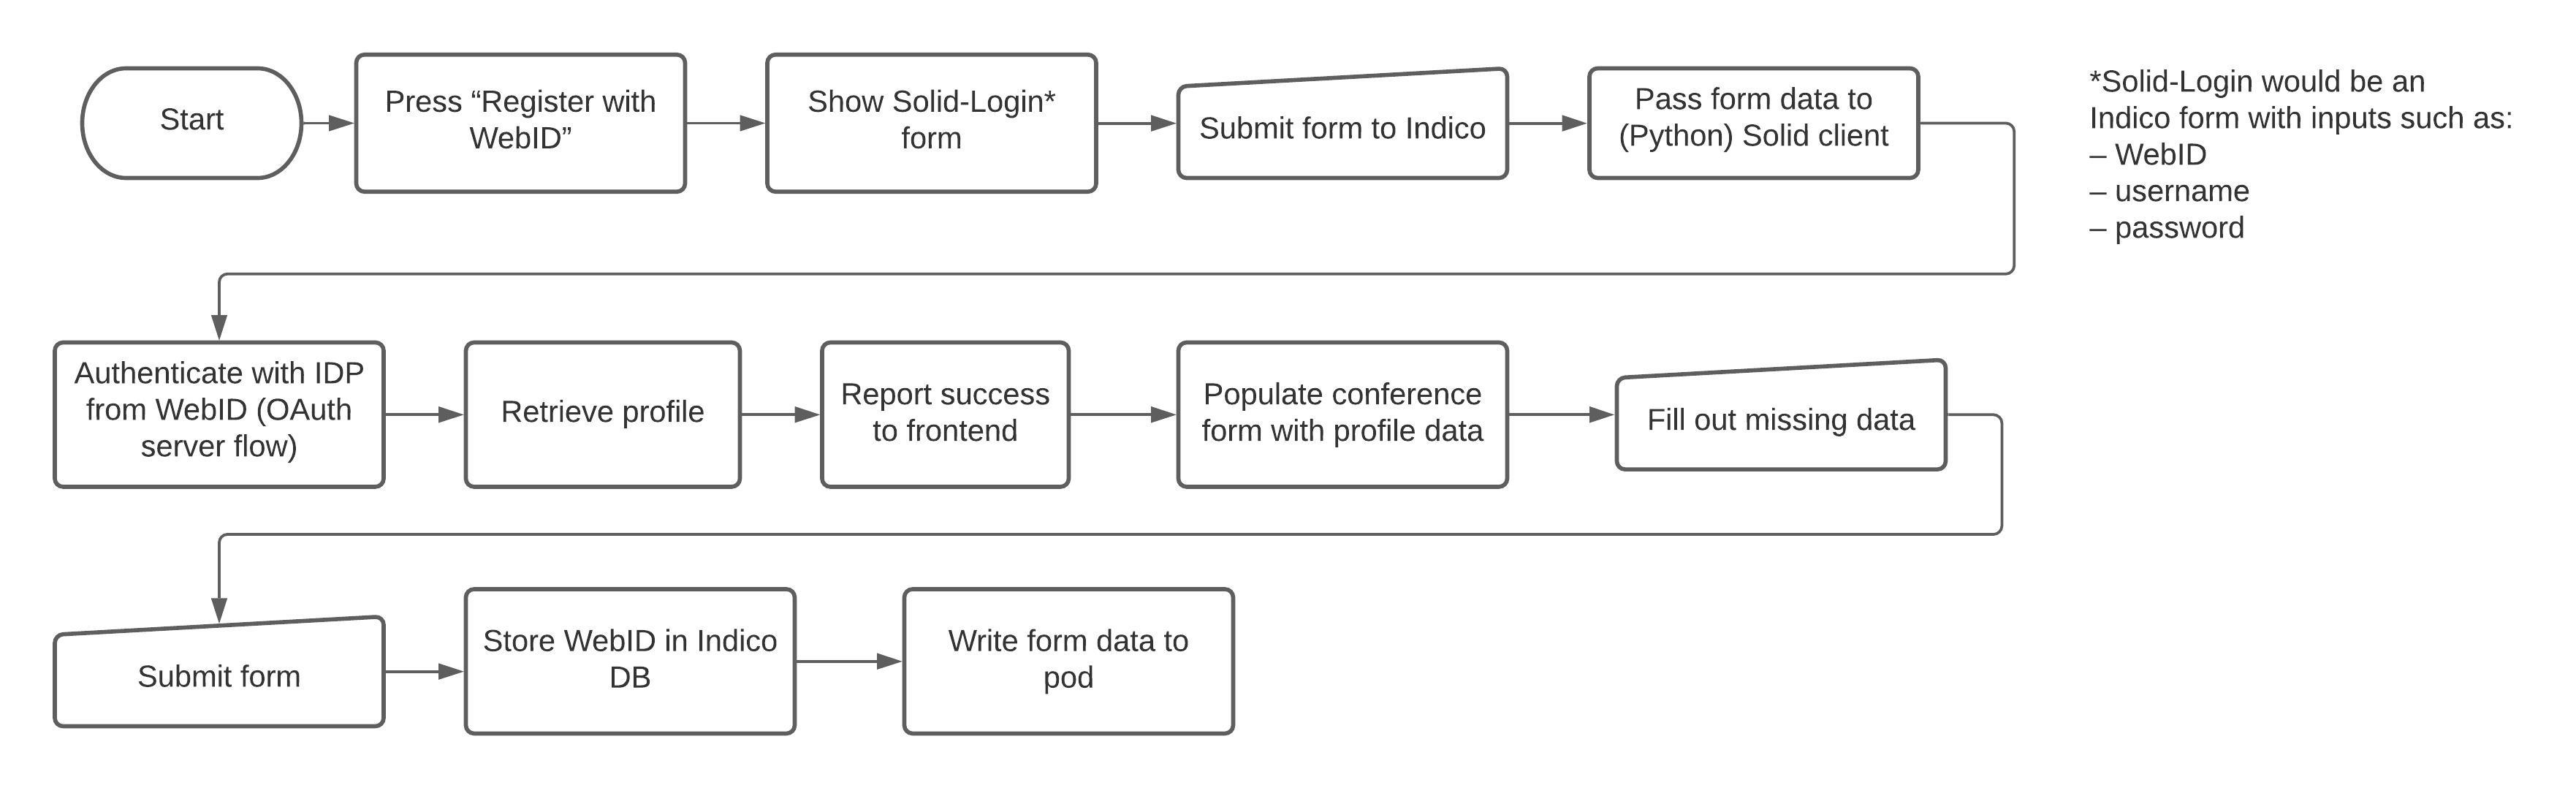
\includegraphics[width=0.6\textwidth]{prototype/graphs/poc-conference_registration_flow-server_side-sideways.jpeg}
    \caption{TODO:}
    \label{fig:poc-conference_registration_flow-server_side-sideways}
\end{figure}

\begin{figure}
    \centering
    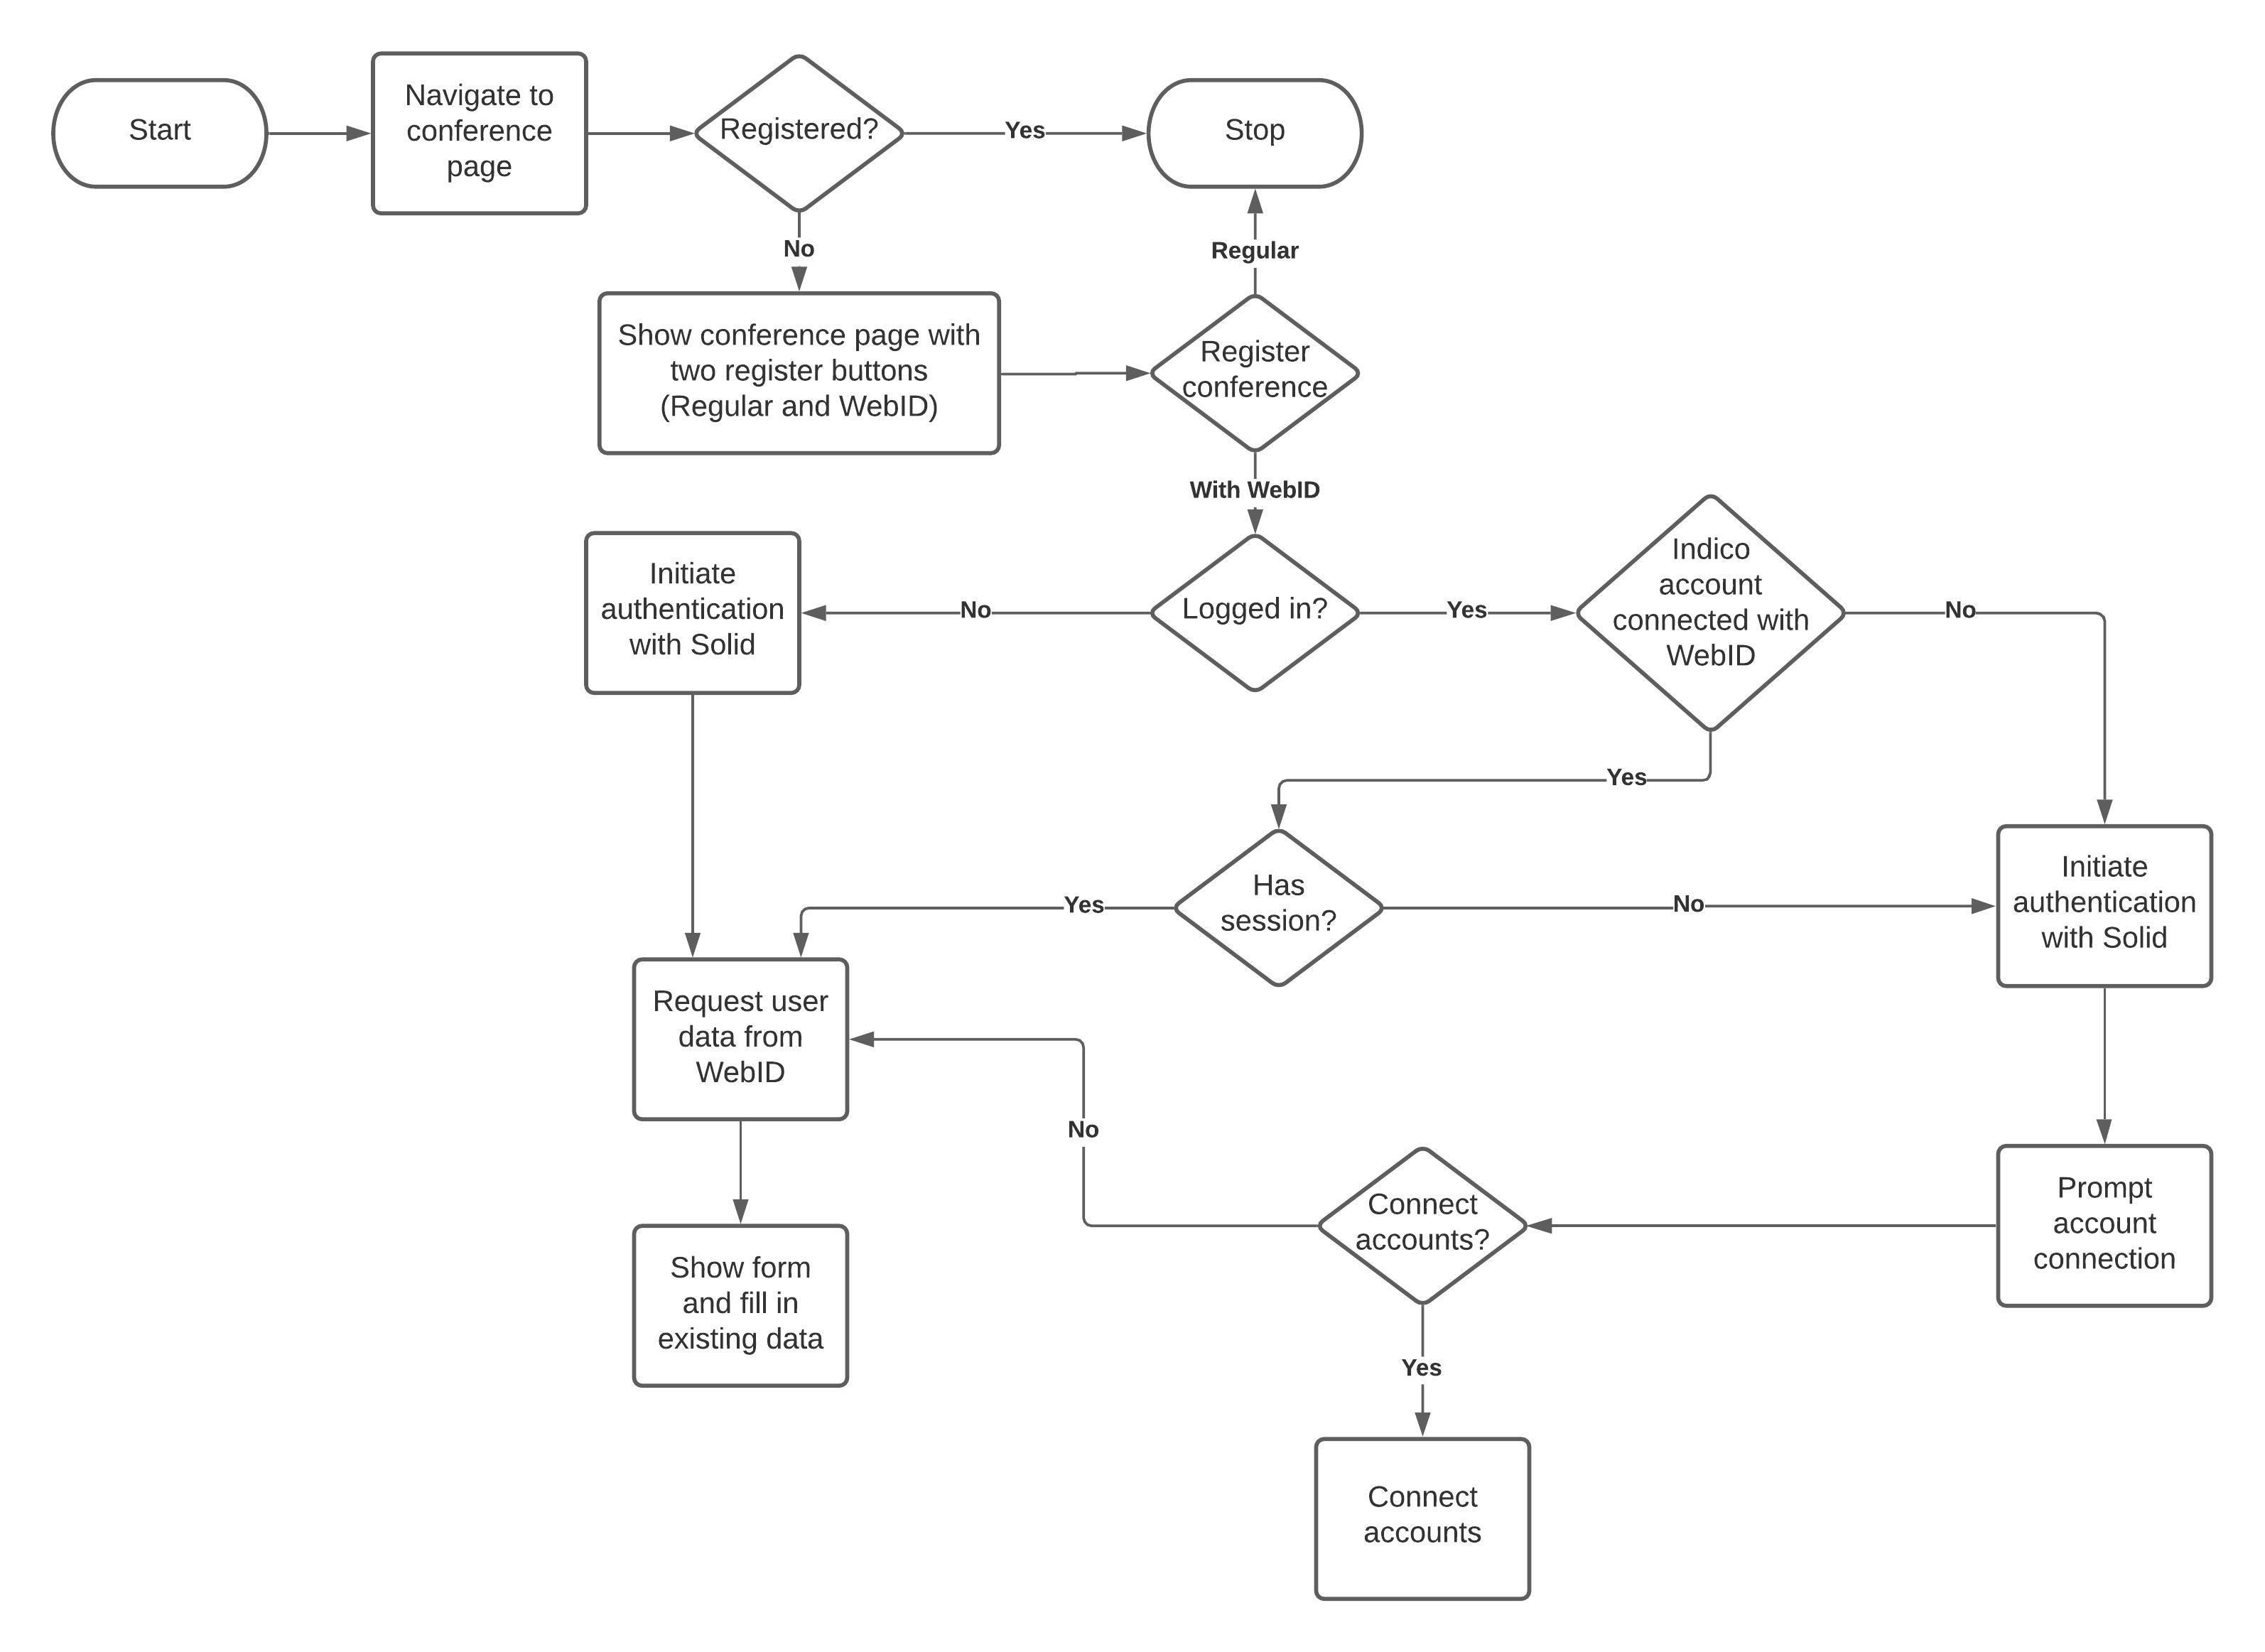
\includegraphics[width=0.6\textwidth]{prototype/graphs/poc-conference_registration_flow-sideways.jpeg}
    \caption{TODO:}
    \label{fig:poc-conference_registration_flow-sideways}
\end{figure}

* Gave up usage control
  * Why it didn't work, and **what is necessary to make it work**
    * usage control
    * question the choice of Indico usage control
    * versioning of tag of personal data
* high-level constraints
* implementation
  * indico limits this
* if indico in this way or more generally

\paragraph{Modification of Resource From Data Pod}\mbox{}\\

\paragraph{Payment on Input Fields}\mbox{}\\

\paragraph{Performance of Large Conference}\mbox{}\\

\paragraph{Availability of Crucial User Data}\mbox{}\\

\subsubsection{Integration With Indico}\mbox{}\\

\paragraph{Bind to Dynamically Created Form}\mbox{}\\

\subsubsection{Evaluation}\mbox{}\\

\paragraph{Metrics}\mbox{}\\
\paragraph{Levels}\mbox{}\\
\paragraph{Components}\mbox{}\\

\subsubsection{Analysis}\mbox{}\\

* performance?
* Management part of Indico
  * Forward data between people
  * **Also serve data to people (admin of registration)**
* Comments are more clear tied to comment

* the flow of Solid (ref Tim from White Area) notifying for future conference